\documentclass[12pt,fleqn,leqno,letterpaper]{article}
\usepackage{graphicx}
\usepackage{hyperref}
\usepackage{booktabs}
\usepackage{textcomp}
\usepackage{gensymb}
\usepackage{float}
\graphicspath{{../figures/}}

\title{Luminosity}
\author{Cameron, M. \and Rosales, V. \and Westermann, J.P.}

\date{July 30, 2017}

\begin{document}

\maketitle
\newpage
\tableofcontents
\listoffigures
\listoftables

\newpage

\begin{section}{Introduction}
  \begin{subsection}{Summary}
    Multiple economic publications have established night-time luminosity as a valid proxy for economic activity. Building on these results, we use night-time satellite imagery with institutional natural disaster records to study the connection between such disasters and economic activity. We attempt to model light intensity over time and find the short- and long-term effects of catastrophe events on economy and infrastructure. In order to achieve these goals, we also plan to build the technical infrastructure for working efficiently with this specific dataset.
  \end{subsection}
  \begin{subsection}{Literature Review}
    \begin{subsubsection}{Luminosity-based Approach}
			The use of night time light data is increasingly being used in economic papers. The aim is to improve the quality of economic data, especially in many poverty-stricken and war-torn countries where it is poor. This data becomes even more difficult to work with once regional economic statistics are needed. It is incredibly difficult to understand the country's economic growth without this information. Light data is seen as a promising development in this area. Not only does it provide information for every country, but it also shows the spread of activity throughout each country and region. Throughout this paper light levels are used as a proxy for the GDP of an area, but is it feasible to use this variable as a proxy? \\
      The paper \textit{``The Value of Luminosity Data as a Proxy for Economic Statistics''} \cite{lightasproxy} closely examines this assumption. Using the same satellite light images as used in this paper, the paper compares light levels to actual GDP data. The light data is aggregated to a $1\degree\times 1\degree$ are to match the finest economic data available to them, although country level data is also examined. The paper concludes that, although the light data can be quite noisy, it provides a good proxy for GDP. Especially in poor countries with poor economic data. In richer countries with much more detailed statistics, because of this noise in measurements it will not provide improvements to the statistics that have already been collected.\\ 
      These arguments are reiterated in the article \textit{``LIGHTS, CAMERA ... INCOME!''}  \cite{lightcamera}. The authors point to the large discrepancy found between national accounts GDP per capita and household survey means, both of which are used to study poverty and growth. I their argument for the use of light data they state that `We think that nighttime lights most likely reflect lighting in houses, production facilities (stores, factories, ports) and modes of transportation. Since nighttime lights data is collected through an impersonal, nonintrusive process, concerns about nonresponse do not apply'. With so much economic data, used in many papers, gathered from surveys, especially in poorer countries, this provides a further argument for the use of light data in this field. \\ 
      The correlation between light levels and economic activity is shown in several revealing ways in the paper \textit{``Measuring Economic Growth from Outer Space''} \cite{growthlights}. The examples used in the paper are the stark contrast on the Korean peninsula of the growth rates north and south of the border. A further example is in Indonesia before and after the Asian financial crisis in 1997. Actual GDP levels are are mirrored by the predicted levels from the light data through the shock. The same can be seen during the genocide of Rwanda. This is an important example as it shows how lights are affected by a shock. Our paper also investigates economic levels after a shock, but this shock is a natural disaster rather than a financial crisis. \\
      Light data has been shown to act so well as a proxy for economic development it is now widely used as such in papers. \textit{``Pre-colonial Ethnic Institutions and Contemporary African Development''} \cite{africalights} finds that the complexity and hierarchical structure of pre-colonial ethnic institutions correlate significantly with contemporary regional development. The paper utilises satellite light data, in particular its property of providing useful economic data for less developed regions, for these findings. This shows how the literature no longer simply considers light data as a promising means of estimating economic activity, it is now actively being used as this measure in the literature. 
    \end{subsubsection}
    \begin{subsubsection}{Natural Disaster Economics}
      TODO Viviana: obviously, as the expert.
    \end{subsubsection}
  \end{subsection}
\end{section}

\begin{section}{Data}
  \begin{subsection}{Data Description}
		The light data used is from the U.S National Center for Environmental Information. This provides an image of the night time lights yearly from 1992 until 2013. Each image is a cloud-free composite made using all the available archived satellite smooth resolution data for each calendar year. In some of these years there were two satellites collecting the light data. For these years, two composites were produced. Several constraints were put on the images for them to be used in the composition to ensure that only the highest quality data was used. These constraints included the solar elevation angle, to ensure there is no glare or sunlit data, and thermal band data combined with surface temperature grids, to detect the presence of clouds. This data is used widely in any papers examining light levels. \\
    Data on natural disasters was taken from The International Disaster Database. The Emergency Events Database (EM-DAT) was the most complete dataset of natural disasters we found. In total it contains the occurrence and effects of over 22,000 mass disasters in the world from 1900 to the present day. Here, we mainly look at earthquakes and since our light data is from 1992 to 2013, we restrict our disasters to earthquakes from this time period. Even with these restriction the dataset has 674 earthquakes. For each of these events we have all of the cities affected, the date of the disaster, the damage caused and the number of casualties and fatalities. From the perspective of cities, we have over $2700$ EM-DAT is used widely in academic publications studying natural disasters of all types.
  \end{subsection}
  \begin{subsection}{Data Preprocessing}
    \begin{description}
      \item[Volume]{While the number of observations is extremely low, as only annual images are available from 1992 to 2013, the dimensionality of each observation (image) is considerable. With a size of $16801$ by $43201$, every image contains $725820001$ pixels in total, which results in more than 700MB of disk-space required for only one image in uncompressed format. This also means that computations on the entire dataset are not possible with common personal computing architecture.}
      \item[Diverse Sources]{To aggregate meaningful information to use in the model, such as economic indicators from the world bank (gdp, import, export, inflation, etc.), we need to join data from a lot of different sources on different aggregation levels.}
      \item[Image Format]{As the data comes in image format, we need to find an appropriate numerical representation of the images.}
    \end{description}
	\begin{subsubsection}{Georeferencing and QGIS}
			In order to georeference the cities, we used the ``Easy Georeferencer'' software, which takes as input the names of the cities along with their countries, and returns the coordinates of the city. After checking that the allocation was correct, we proceed to estimate the number of disaster per year and region. \\
			QGIS is a geographic information system application that supports viewing, editing, and analysis of geospatial data. It is used widely by geophysicists, geographers and many other areas using geospatial data. The advantage of using QGIS for our data is that we are able to merge geographic layers. We use three layers for our models: the nighttime light images, polygons in the shape of each region and the points of each city affected by an earthquake. Overlaying these images and merging them gives a map, where each point on the globe has the value of the light level, which region the point is in and the location of cities affected by earthquakes.   
			\begin{figure}[htbp]
			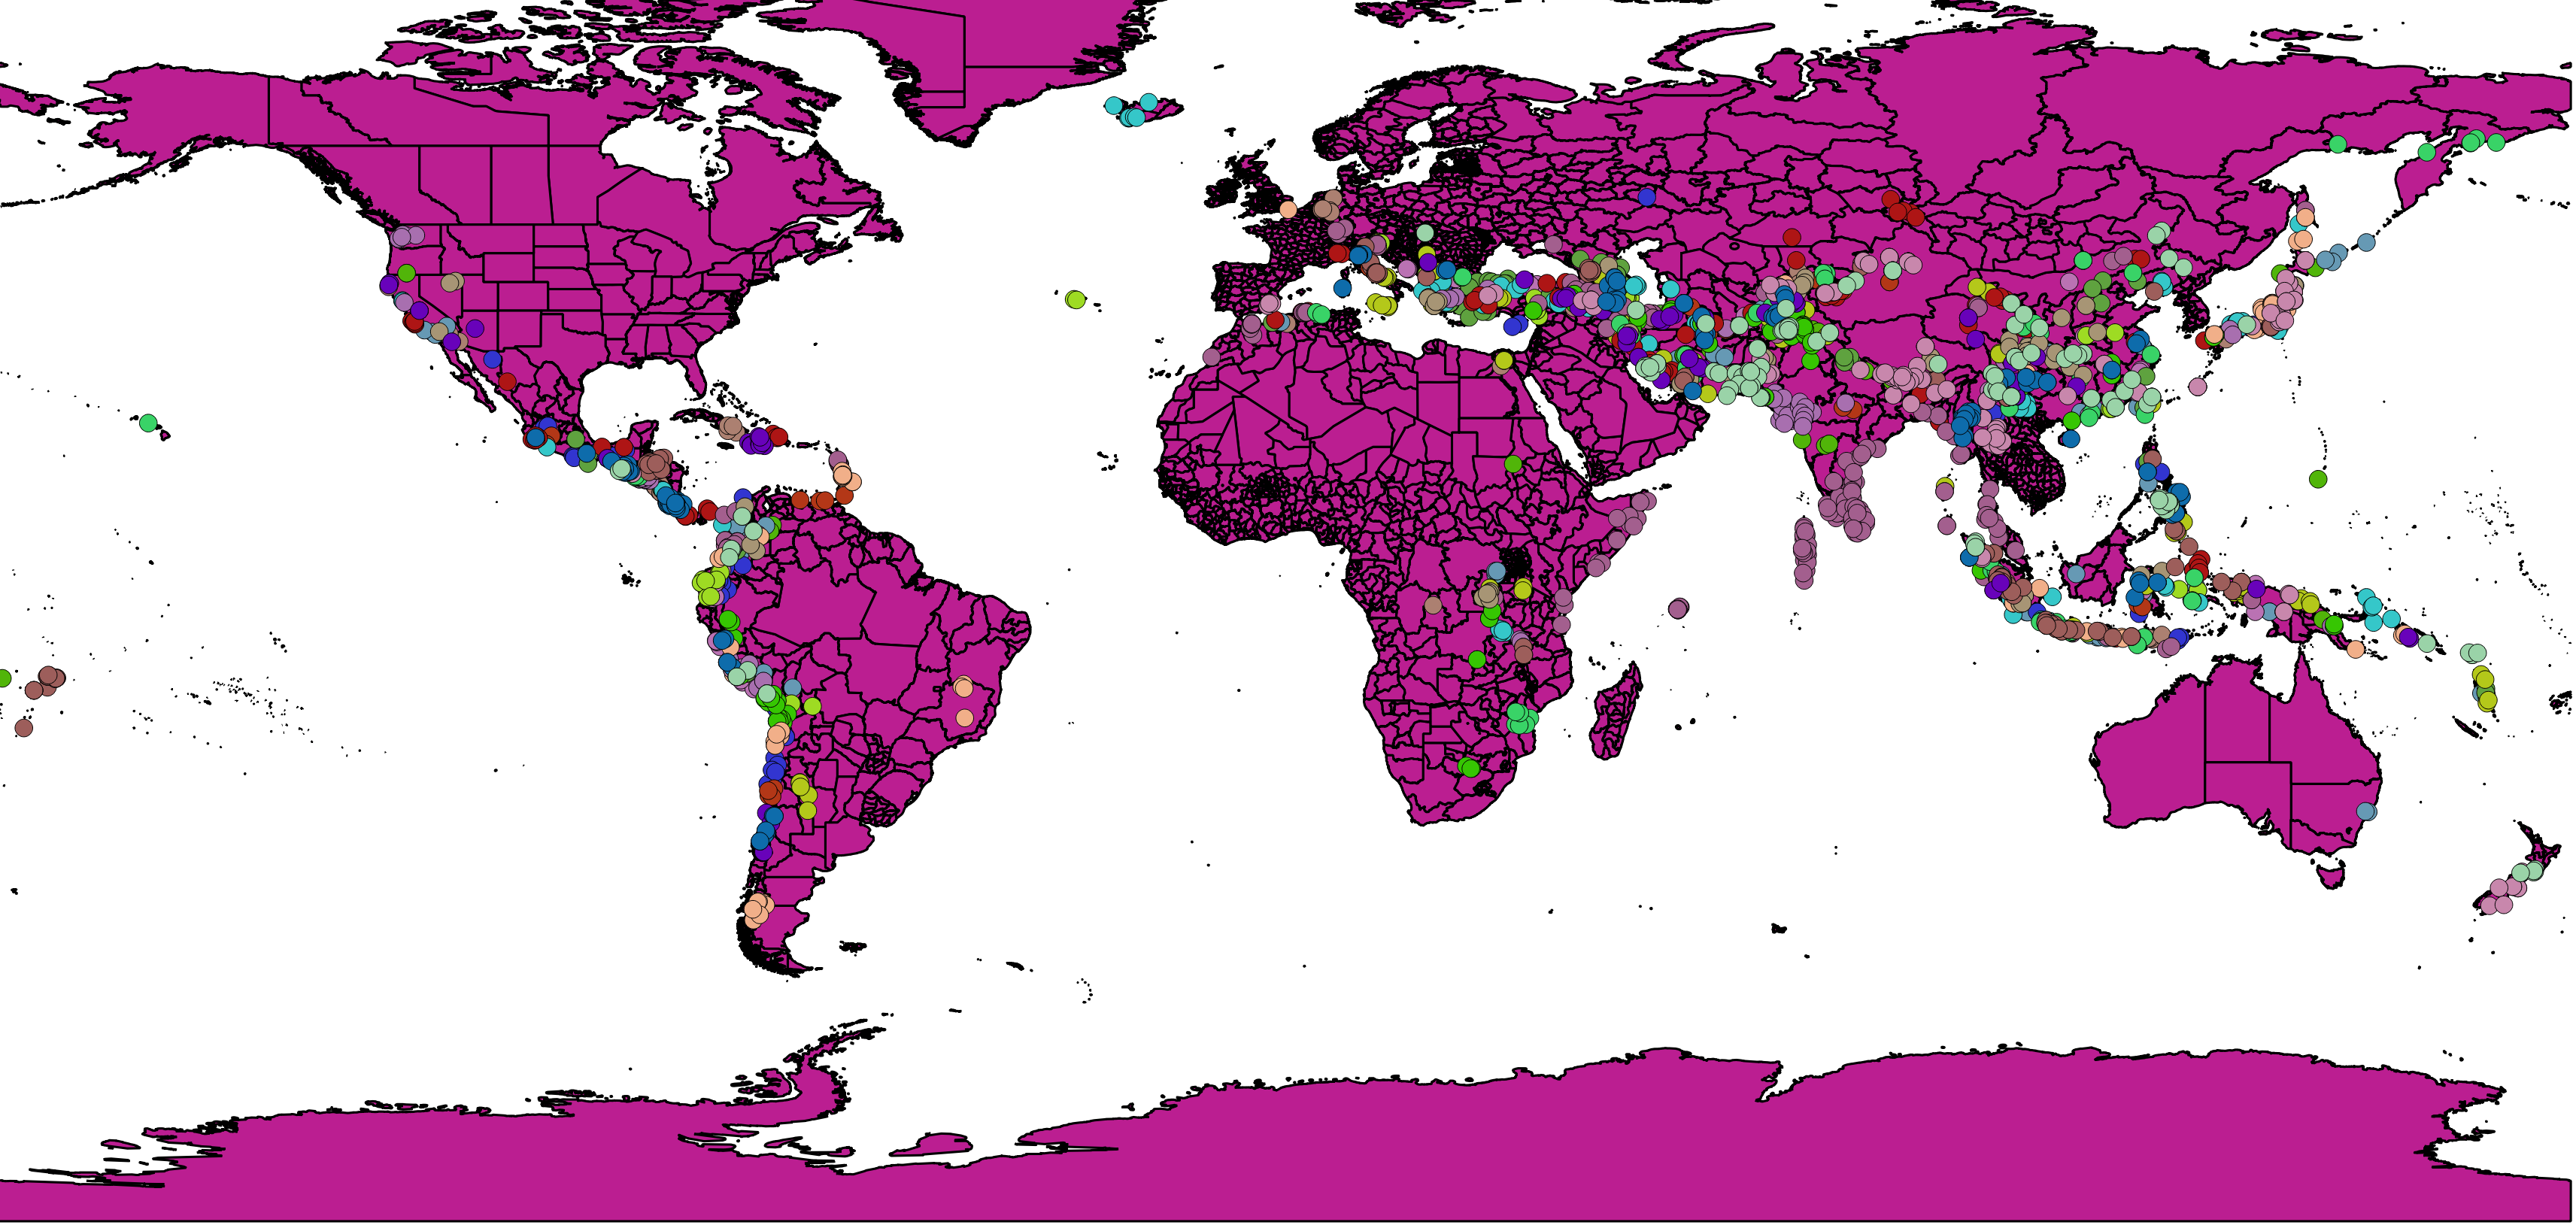
\includegraphics[width=1\linewidth]{world_regions.png}
			\centering
			\end{figure}
			This is a snapshot summarising two of the layers that we are working with, namely the polygon layer and earthquake data points. The image shows every earthquake from the EM-DAT database within the time frame of the light images we have.
    \end{subsubsection}
    \begin{subsubsection}{Python Architecture}
      To enable exploration and flexible modelling of the data even on a platform where memory and computing power are quite restricted, we built a supporting architecture in python for loading the images and aggregating the features.
      To quickly load entire time series of the most important places, the sections of the image representing the biggest cities and a 300x300 area around them are cut out and stored as seperate time series. This allows for more easilty training predictive models for the luminosity.
      Additionally, functions where created to easily load a 'section' time series (the series of images for one particular subsection of the world's image), given coordinates and the desired size of the image.
      The stored data is no longer in the \textit{tif} format provided at download. All images have already been passed into arrays and stored as compressed numpy arrays. That reduces the required storage space by an order of magnitude.
      The functions to preprocess and load the data can be found in the \hyperref[www.github.com/westermann/luminosity]{GitHub repository}. To make sure that the code doesn't throw a \textit{MemoryError} or similar when working on a less powerful machine, most of these functions have been optimized to free up memory space as fast as possible and always only work with one single memory mapped full-size image array.
    \end{subsubsection}
  \end{subsection}
\end{section}

\begin{section}{Modelling}
  \begin{subsection}{Disaster Impact Models}
    Exploratory analysis and some basic models are a first step to assessing the impact of natural disasters on the luminosity time series. For this, we need to make a modelling decision regarding how the disaster (represented only as a single point location) can be geospatially associated with pixel luminosity values. In the following we will quickly introduce and discuss two different approaches to this problem, one that is less conservative and one that complies with most of the research currently published in the area.
    \begin{subsubsection}{Linear Distance-based Modelling}
      One practical mathematical choice is a function decaying with distance affecting areas or even individual pixels on the grid. The advantage of this method is that it is simple to explain, easily tuneable and leaves a lot of flexibility for modelling. Additionally, it captures the notion that areas in the vicinity of a disaster event are more likely to be affected than those further away by default.
      We trialed this approach using the luminosity data in combination with location-tagged earthquakes from the U.S. Geological Service. We extracted 150x150 squares from the satellite image of the entire planet in a similar fashion as a convolutional neural network would apply to an image. Then we filtered the top $t\%$ most luminous 'subimages', as we can generally disregard those parts of the world that contain no lights (oceans, deserts, etc.) and calculate a disaster coefficient based on a function decaying linearly with distance. The $t$ percentage threshold can be tuned in order to keep the data small enough to process. This is necessary as in practice, finding the disaster coefficient means calculating the distance between every image section's center and every earthquake and then applying a linear function of the distance and the magnitude for every earthquake that occurs in a given year. These effects summed up, generate a disaster impact variable for that observation. This results in a high computational load as for every section that we extract from the image, we need to compute the eucledian distance to every singe one of the 25000 earthquakes, making in almost infeasible on a common laptop. However, already only the luminosity growth between beginning and end of the image time series and the disaster coefficient show promising qualities of the data when plotted agains one another.
      \begin{figure}
        \centering
        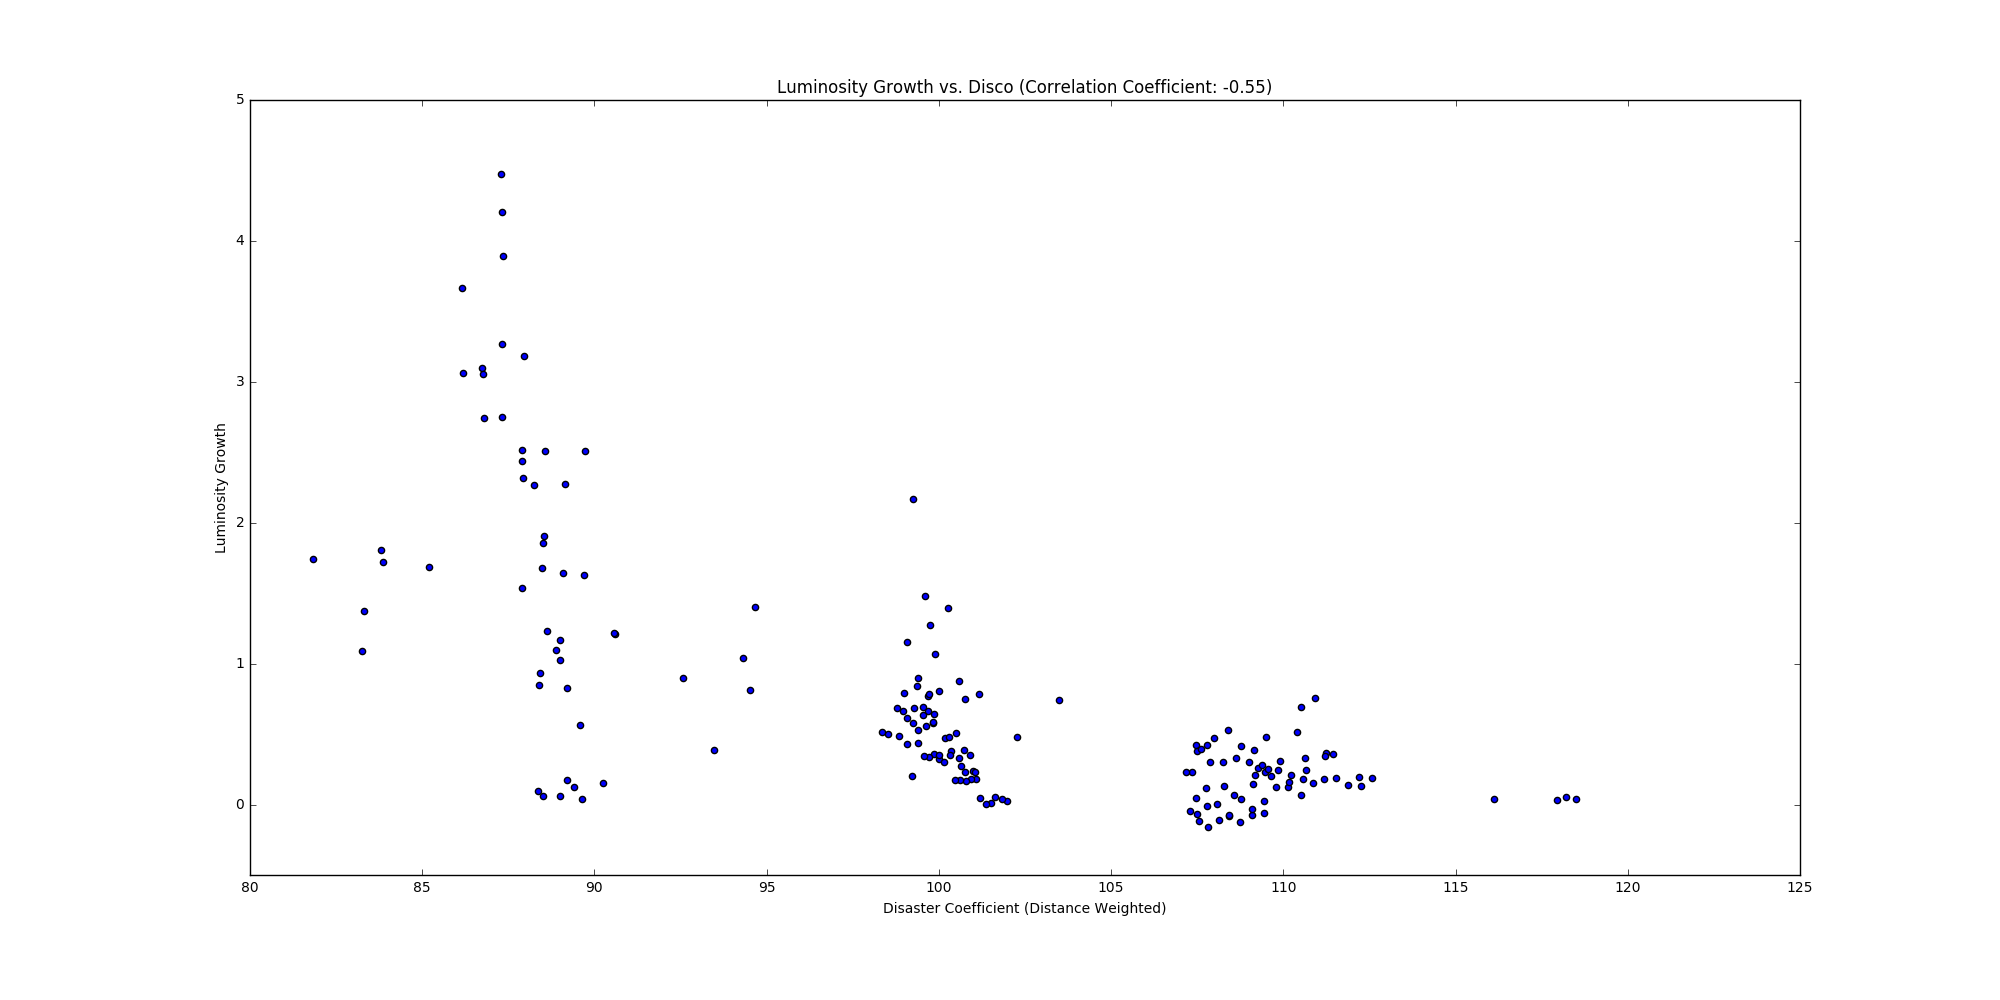
\includegraphics[width=1\linewidth]{linear-lum-vs-disco}\label{fig:linear-model-disco-vs-lum-growth} %TODO: Adjust plot pngs to have sensible size for document
        \caption{Luminosity Growth 1992-2013 plotted against a linearly decaying disaster coefficient for 150x150 image sections.}
      \end{figure}
      As we can see, there is a negative relationship between (luminosity) growth and the impact of earthquakes. The effect has been aggregated over the entire series and we can thus look at this as just showing the general implications for growth of a city/region by being in or closer to an area that has more earthquakes. It is notable that not necessarily the actual growth value, but the variance of the growth values strongly increases for areas less prone to earthquake effects.\\
      However, this approach makes some strong assumptions about the nature of natural disasters that don't hold in reality. An important factor in how much impact a disaster has on a region are geographical features: An earthquake will affect different areas differently based on their rockbed and geological consistency while e.g.\ storms and floods depend strongly on the topography. Nevertheless, the calculation of such a disaster coefficient yields promising results and suggests there is a relationship in the data between disaster coefficient and the growth in a location, proxied by luminosity.
    \end{subsubsection}
    \begin{subsubsection}{Recorded Disaster Impact-based Modelling}
      Another possible approach, one that is far more commonly applied in Economics, is to use institutional data on which cities where affected by an earthquake. Using the EM-DAT international disaster database, we can obtain records of cities that were affected by a given earthquake in a given year. Matching this with a simple list of the world's largest 50000 cities, we can obtain a panel dataset that associates earthquake damage without any measure of magnitude to cities, some affected, others not.
      Using this dataset and calculating luminosity sums for each of the areas around a city, we can fit a simple vector autoregression model to explore the impact of earthquakes on these time series. The model is enriched with economic indicator values as well as import and export statistics and fit for every city indipendently. To get a general overview of the relationship between luminosity and the disaster events, we can simply average the earthquake lag coefficients for all models. Doing this yields the following average coefficients (the distribution of which can be viewed in Figure TODO.\\
      \begin{center}
        \begin{tabular}{lr}\\
          \toprule
          {} & Average Coefficient \\
          \midrule
          el1 & -0.60 \\
          el2 & -0.37 \\
          el3 & -0.14 \\
          \bottomrule\\
        \end{tabular}\\
      \end{center}
      \begin{figure}
        \centering
        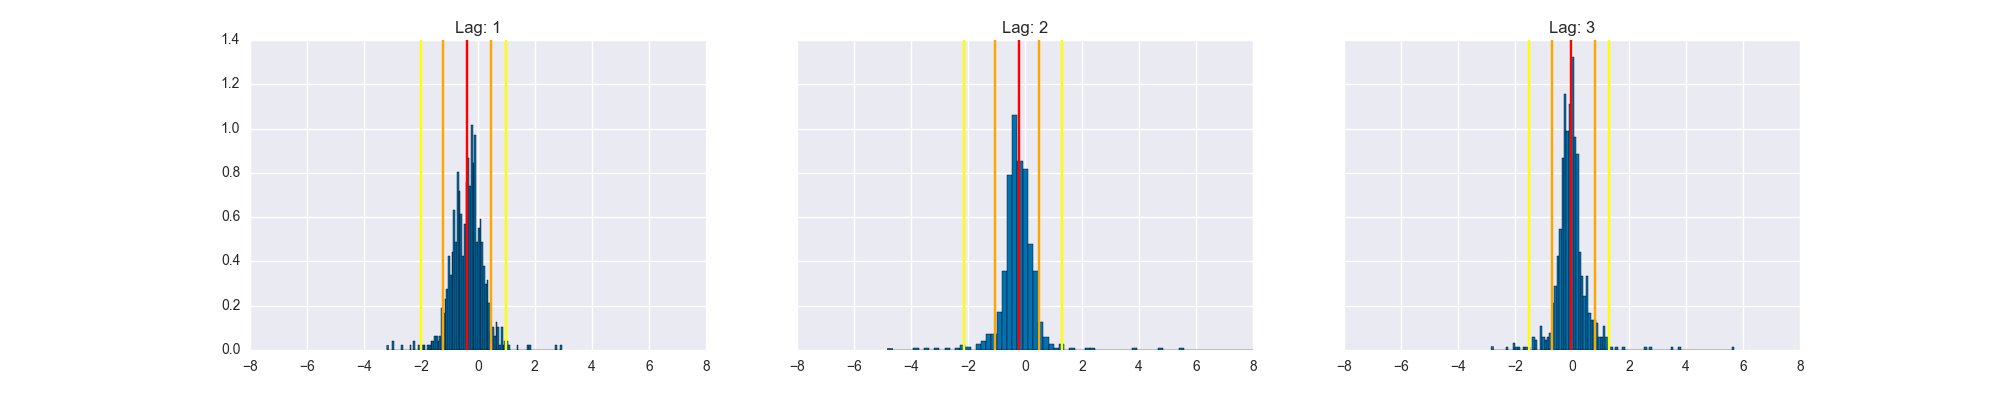
\includegraphics[width=\linewidth]{non_balanced_earthquake_coefficients_distribution}\label{fig:non_balanced_earthquake_coefficients_distribution} %TODO: Adjust plot pngs to have sensible size for document
        \caption{Distribution of Lag Coefficients for Earthquakes in Vector Autoregression Models per City with 95th and 99th Percentiles}
      \end{figure}
      These results support those found using the alternate approach, that there is a measurable effect of earthquakes on the summed luminosity for an area. As the distribution of the lag coefficients suggest, the impact is far stronger in the first year and decayes quickly in the second and third as things normalize. As these coefficients are aggregates, however, they do not provide much information on the significance in a specific case or the detailed recovery process. Nevertheless, these preliminary results in combination with those collected using a distance-decay impact model, are important baselines for a more elaborate panel model.\\
      While being based on fewer assumptions about the nature of a distaster's impact radius and magnitude due to using human assessment-based data in every case, this approach has an obvious shortcoming the alternative did not: As we do not imply any kind of decay with distance from the earthquake location or use information on the earthquake location and magnitude at all, we are entirely neglecting the intuitive notion that the impact of the earthquake differs from place to place. Because of these shortcomings, future research should utilise a combination of the two approaches, using also distance from the earthquake for any given city as part of the function that describes disaster impact.
    \end{subsubsection}
  \end{subsection}

  \begin{subsection}{Panel Model}
    \begin{subsubsection}{Region-based Panel}
      TODO Viviana
    \end{subsubsection}
    \begin{subsubsection}{Section-based Panel}
      Using the list of cities affected by earthquakes created from the EM-DAT disaster database, we can construct a panel dataset containing all years available (1992-2013) and a selection of the world's most populous cities. To achieve this, we simply take a 50x50 pixel square around the city's coordinates to calculate the luminosity. This can be combined with the other data described in the previous section to form a more granular panel that can study effects on a city level, rather than the very aggregated regional level. The advantage of this method is also that time-series constructed from city locations are more homogenous than those constructed on regional level. For an overview of what the time series used with this methodology look like in terms of the actual image who's luminosity is summed up, you can refer to Figure TODO.\\
      \begin{figure}
        \centering
        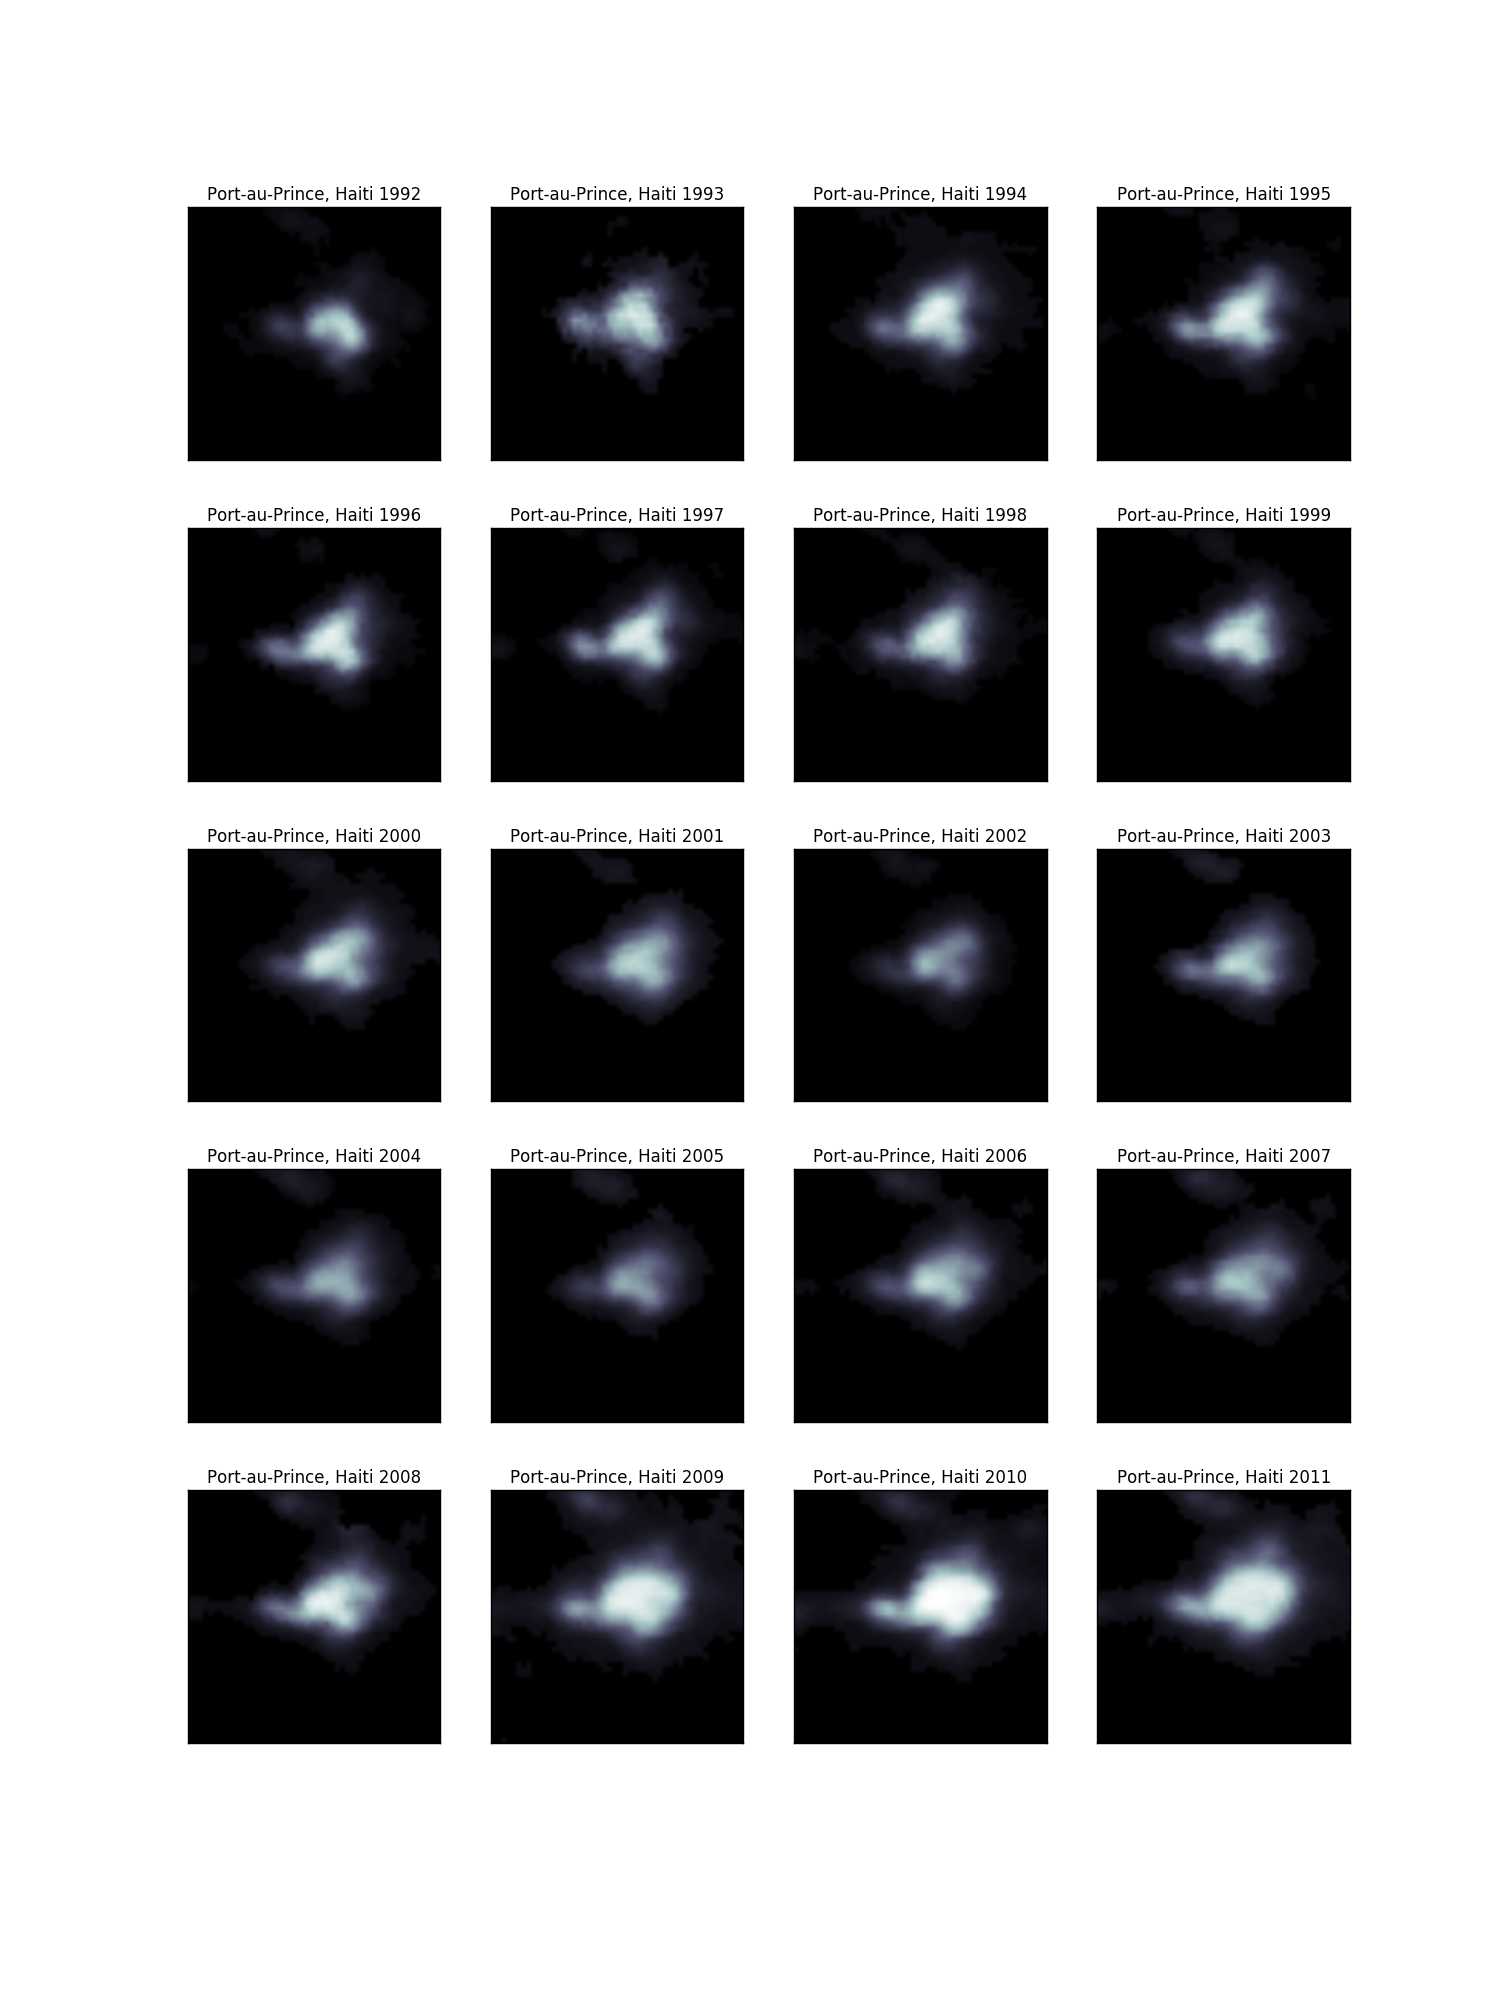
\includegraphics[width=\linewidth]{haiti_luminosity_series}\label{fig:haiti_luminosity_series}
        \caption{50x50 pixel atellite image cutout of Port-au-Prince, Haiti}
      \end{figure}
      A possible extension to this methodology that is beyond the scope of this paper, would be to extract the actual individual settlements, thus ignoring surrounding locations that are simply included because of the frame size and shape.
    \end{subsubsection}
    \begin{subsubsection}{Dynamic Panel}
      TODO Viviana: Describe here how the model that you are using is constructed, where you got it, etc.
    \end{subsubsection}
  \end{subsection}
\end{section}

\begin{section}{Results}
  \begin{subsection}{Case Analysis}
    % \begin{subsubsection}{Income-dependent Disaster Recovery}
    %   We can also attempt to analyse how the recovery process after an earthquake affects regions in different ways depending on their other characteristics. One of the splits that come to mind is by income level of the respective countries. This can potentially show disparities in how the earthquake event is handled dependent on the country's general economic situation and development level. Figure TODO shows the average earthquake lag coefficients for different income groups.
    %   \begin{figure}
    %     \centering
    %     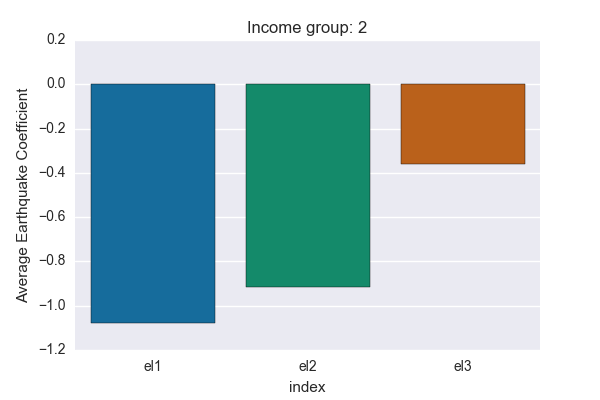
\includegraphics[width=.5\linewidth]{non_balanced_earthquake_coefficients_income_class_2}\label{fig:non_balanced_earthquake_coefficients_income_class_2}
    %     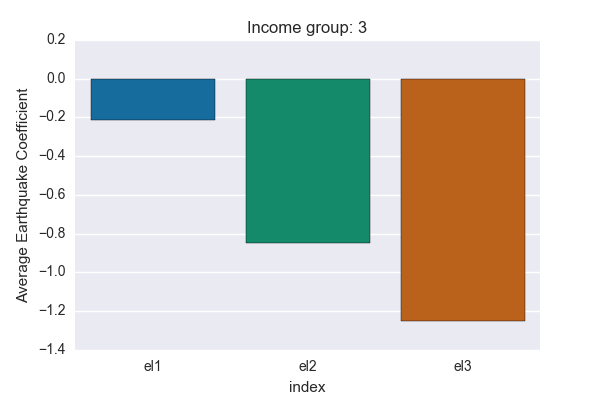
\includegraphics[width=.5\linewidth]{non_balanced_earthquake_coefficients_income_class_3}\label{fig:non_balanced_earthquake_coefficients_income_class_3}
    %   \end{figure}
    %   The 
    % \end{subsubsection}
    \begin{subsubsection}{Tocopilla and Maule Earthquakes}
			In 2007 an earthquake of magnitude 7.7 hit Tocopilla in the more prosperous north of Chile. 3 years later and an 8.8 magnitude earthquake devastated the poorer Maule region. While Tocopilla, in the Antofogasta region, is the highest ranked Chilean region by GDP (PPP) per capita this contrasts to Maule being the third lowest in Chile. While both earthquakes caused serious destruction in both areas, we try to examine the recovery of each region. To compare the effects of the two earthquakes, it is estimated that 14.8\% of the population in Tocopilla were left homeless by the disaster in 2007, while in Maule in 2010 this figure is estimated at 20.4\%, figures from the Casen Post-Earthquake Survey. We aim to find, using our light data, if the more prosperous region recovers from the destruction at a quicker rate. \\
			\begin{figure}[H]
        \centering
				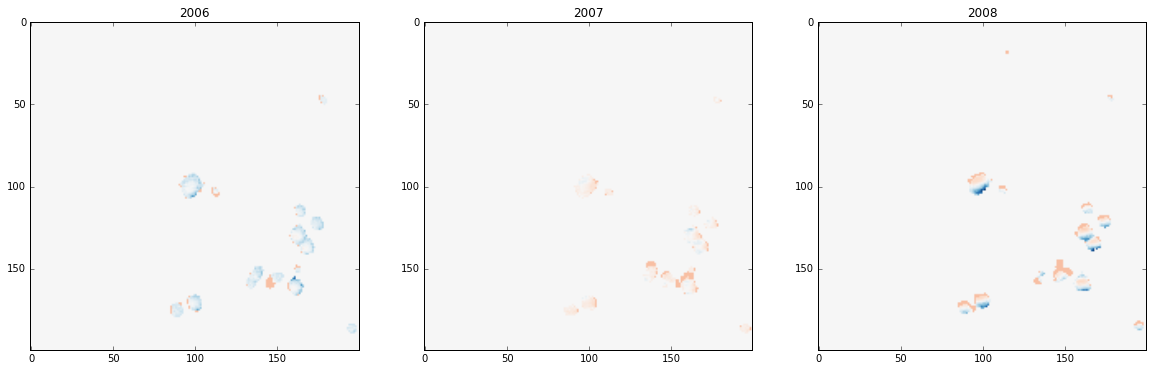
\includegraphics[width=1\linewidth]{tocopilla_series}\label{fig:tocopilla_series}
				\caption{Absolute change in luminosity in Tocopilla}
				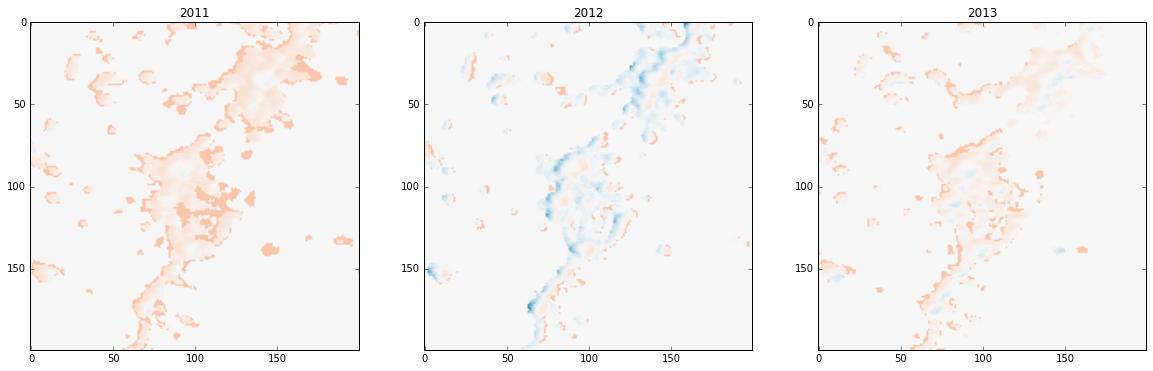
\includegraphics[width=1\linewidth]{maule_series}\label{fig:maule_series}
				\caption{Absolute change in luminosity in Maule}
			\end{figure}
			From simply looking at the images of Tocopilla, it is quite difficult to observe the effects of the earthquake from the light differences. While the 2010 earthquake in Maule shows much clearer effects. As expected we have the immediate decrease in luminosity, represented by red, following the earthquake. Followed by a bounce back, in blue, the following year. \\
			\begin{figure}[H]
			\centering
				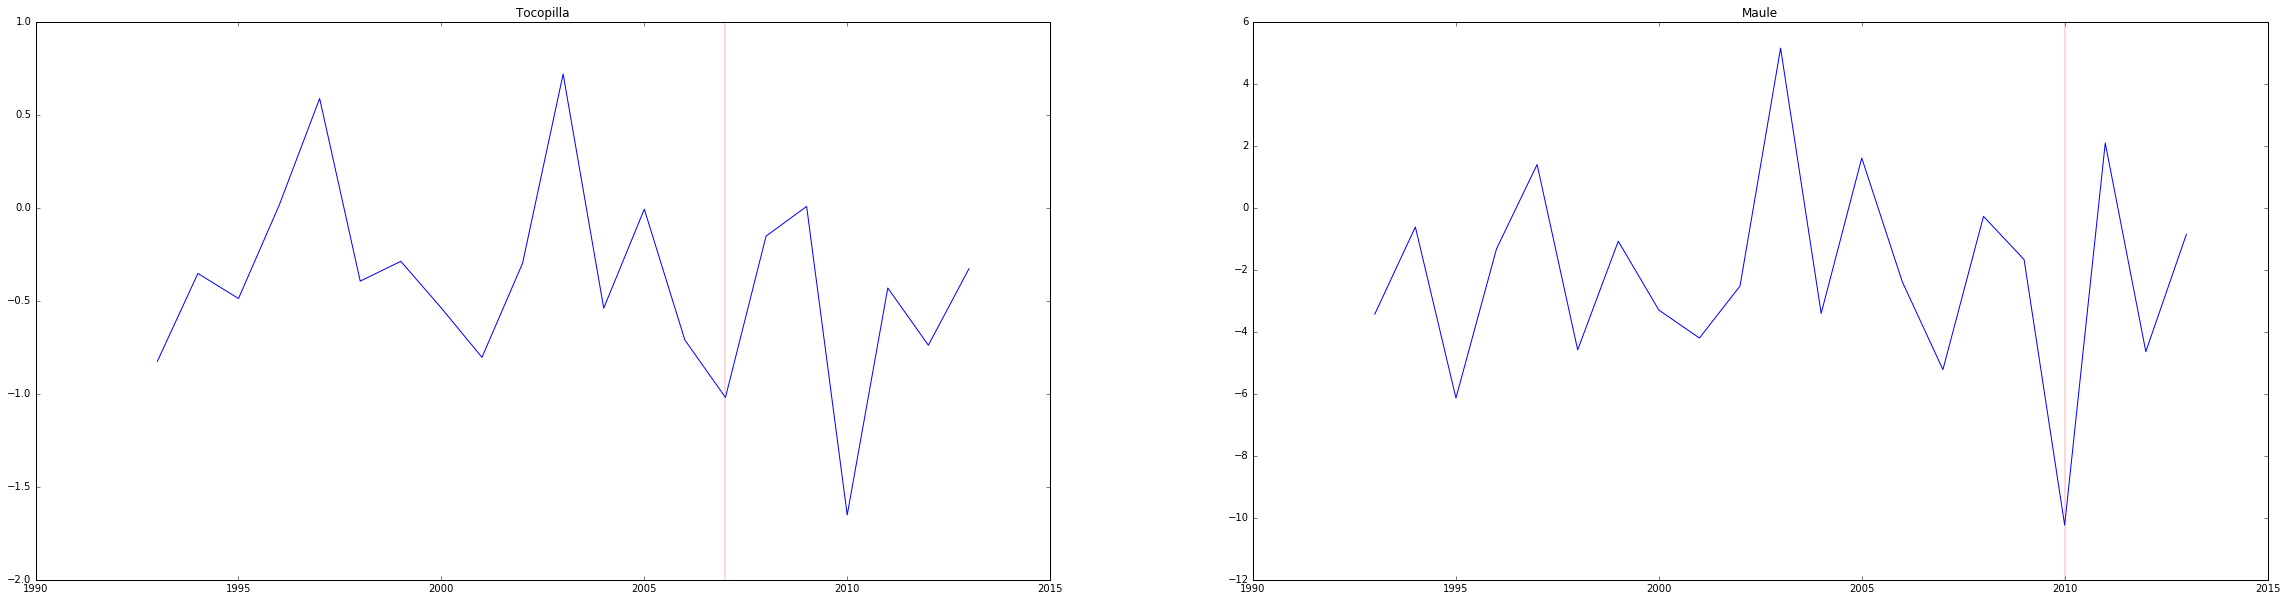
\includegraphics[width=1\linewidth]{maule_tocopilla}\label{fig:maule_tocopilla}
			\end{figure}
			These two graphs show the absolute change in the mean luminosity of the areas over time, with the red line indicating the time of the earthquake. We can see that the 2010 disaster in Maule had a much larger effect on light levels in the region than in the Tocopilla quake. Despite this huge drop in light levels, in the year following the disasters both areas see recovery. In the case of Tocopilla, the mean luminosity drops by 0.06195 in the year of the earthquake and in the following year it grows by 0.01415. While in the case of Maule, the mean light levels drop by -0.873175 and recovers by 0.403875. Although the magnitudes of the variations are of different sizes in the two cases, we can see that Maule regains a larger proportion of its luminosity than Tocopilla. This is interesting as it would have been reasonable to expect the more prosperous region of Tocopilla to recover more of its light however, this is not the case. One explanation for this could be the humanitarian aid provided. In 2010, one week after the earthquake, Chile formally requested international aid. The earthquake and following tsunami in Maule caused a many more deaths and much more destruction, as can be seen in the larger drop in light levels. The number of fatalities attracted much international attention, and in turn aid. This could be one explanation for the recovery of the Maule region. \\
			However, we can note that the earthquake in Maule caused a serious outlier in the drop in lighting, this is not the case in Tocopilla. Tocopilla actually has a larger drop in luminosity in 2010, when there is no earthquake in the region. We can see a shift in the light, with no disasters. How much of this change in light can we attribute to the natural disaster rather than simply the variance in light between the yearly pictures.
		\end{subsubsection}
	  \begin{subsubsection}{Fukushima Daichii Nuclear Disaster}
			On the 11th of March 2011 the most powerful earthquake ever recorded in Japan, a 9.1 magnitude shock, originated 70km off the east coast. This triggered a tsunami with waves reaching 40m tall. When these waves struck the Fukushima Daichii Nuclear Power Plant there were 3 nuclear meltdowns resulting in radioactive materials being released in chemical explosions. \\
			Not only is Fukushima an interesting example of recovery after a serious disaster, but also a prime example of avoidance behaviour. Avoidance behaviour is the act of a person removing themselves from an unpleasant situation. Classic examples of avoidance behaviour would be the movement away from polluted areas, people will avoid pollution when choosing where to live or even their routes to destinations. In the case of Fukushima we effectively have enforced avoidance. Within the first two weeks of the accident all residents in a 30km of the plant were advised to leave their homes. After one month a complete "no-go" zone was introduced around the plant. This "no-go" zone is still in place today. \\
			From the satellite data we aim to investigate several aspects of the Fukushima disaster. The first being, how clearly can the effects of, and recovery from, the meltdown be seen. Another would be, is there evidence of the avoidance behaviour from Fukushima and the surrounding area? 
			\begin{figure}[H]
				\centering
				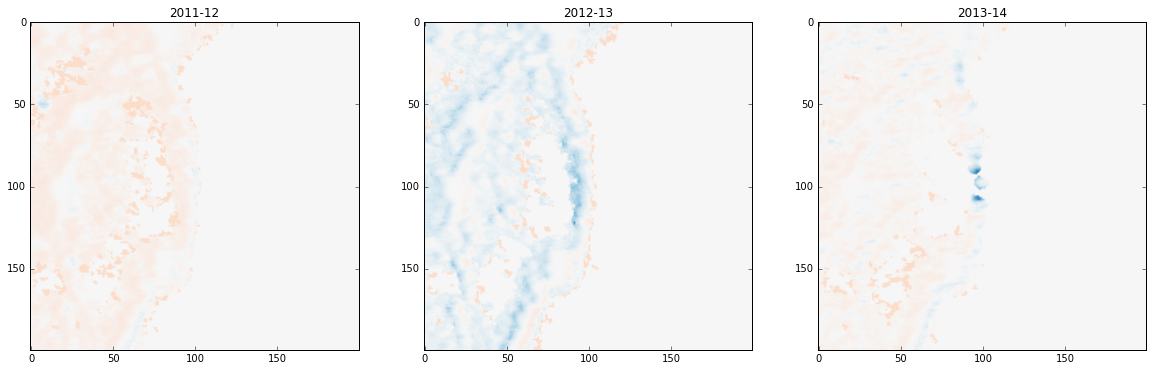
\includegraphics[width=1\linewidth]{fukushima}\label{fig:fukushima}
			\end{figure}
			These images show the change in light levels over the year in the area around the Fukushima disaster with the power plant in the centre. In the images red colouring represents a decrease in the absolute value, while blue shows an increase. A darker colour shows a larger change in light. \\
			The year of the disaster, 2011, unsurprisingly shows almost exclusively red colourings. In 2012, we see an influx of lights to the recovery area. This is common in most of the disasters we have studied. In terms of absolute change in light levels, we find that the Fukushima area recovers almost exactly the same luminosity that it lost after the earthquake. However, we see some rather surprising information from the 2012 image and also the 2013 image. In 2012 we see some of the darkest blue colour in the centre of the image, exactly corresponding to the location of the power plant. This is despite the fact that in 2013, there is still the "no-go" zone and evacuated areas. Perhaps more surprising is the 2013 image. In most of the lit areas in 2013 there is a decrease in luminosity, except in one area, the location of the power plant.  
			Unfortunately the light data only extends to 2013. We can see the devastation and immediate recovery, but we cannot fully see and analyse the avoidance behaviour of the population over time.  
		\end{subsubsection}
  \end{subsection}
  \begin{subsection}{Panel Modelling Results}
    TODO Viviana: Describe the results of the regression here, significant values and what those values mean.
  \end{subsection}
  \begin{subsection}{Conclusions}
    Using luminosity as a proxy for economic activity, we were able to uncover the effect that earthquakes have on the areas they affect. The results show that, as one would expect, the occurance of such an event influences economic growth negative in the coming years. While affects can be found for multiple following years, regression results indicate that only the first-year lag has statistically significant impact. This is in contrast to prior research which failed to link earthquakes to economic development while only finding significant relationships related to meteorological disasters. Additionally, we have provided a technical framework with which it is easy to explore and visualize the satellite images programmatically.
  \end{subsection}
  \begin{subsection}{Outlook}
		The work completed during this thesis creates the basis for many further lines of research. Using the data infrastructure already put in place and the aggregated datasets, it is possible to explore many more aspects of disaster recovery and analysis can be extended to include more diverse natural catastrophe data. The large amount of data available in this field also enables a more granular analysis to fine-tune results of the models in this paper. As most of the light information used is aggregated at different levels, but never used directly, there is potential to uncover more connections between demographic variables, disasters and luminosity. Additionally, the night-time images also contain geospatial information with regards to the impact on a level that would allow to study e.g. following population movements or permanent infrastructural changes due to disaster events. The case studies presented in this paper propose possible research questions that are to be explored in more detail in future work. Additionally, as part of the research work, we constructed different types of predictive models for the luminosity that are based on 'black-box' approaches and are able to estimate next-year luminosity values for image sections with high accuracy. There is potential to use these kinds of models to simulate disaster events and give e.g. economic risk estimates.
  \end{subsection}
\end{section}

\begin{thebibliography}{9}
	\bibitem{lightasproxy} 
	Xi Chen and William D. Nordhausn. 
	\textit{Using luminosity data as a proxy for economic statistics}. 
	Proceedings of the National Academy of Sciences, 2010.

	\bibitem{lightcamera} 
	Maxim Pinkovskiy and Xavier Sala-i-Martin. 
	\textit{Lights, Camera,...Income! Estimating Poverty Using National Accounts, Survey Means, and Lights}. 
	NBER WP 19831, 2014.

	\bibitem{growthlights} 
	VJ Henderson, A Storeygard and Weil DN. 
	\textit{Measuring Economic Growth from Outer Space}. 
	American Economic Review, 2011.

	\bibitem{africalights} 
	Stelios Michalopoulos and Elias Papaioannou. 
	\textit{Pre-colonial Ethnic Institutions and Contemporary African Development}. 
	Econometrica, 2013 Jan; 81(1): 113–152.

	\bibitem{houserates} 
	Chilean Ministry of Planning . 
	\textit{Encuesta Post Terremoto: Principales resultados}. 
	Ministerio de Planificación, 2011.
\end{thebibliography}

\end{document}
